\chapter{Introduction}

%------------------------------------------------------------------------------%
\section{Motivation}  %\label{sec:xx}
%------------------------------------------------------------------------------%

In scientific and engineering contexts, physical systems are represented by mathematical models, which often take the form of partial differential equations (PDEs). These models are characterized by a set of parameters, and since they relate these parameters to states that can be observed, they are referred to as forward models. The forward problem, then, involves solving the PDEs for a given set of parameters. Inverse problems, on the other hand, arise when the parameters are unknown and one tries to infer these parameters based on observations of the states or parameters \cite{Taran05, BanksKuhn89}. Inverse problems appear in many contexts, such as heat transfer \cite{Alif94}, medical imaging \cite{Arr99,Ren10}, contaminant source identification \cite{Sun99}, and reservoir characterization \cite{OliReyLiu08}. 

In such applications the parameters may be numerous, and yet what is ultimately of interest may be some low-dimensional Quantity of Interest (QoI). For example, we may wish to infer the permeability field of an aquifer to form a numerical model that can then be used to design an optimal management policy for the groundwater in the aquifer \cite{Sun99}; in this case, the QoI might be the concentration of a contaminant at a water well resulting from the implementation of a particular policy. In such a situation, where the QoI is of greatly reduced dimensionality compared to the parameters, it may not be necessary to fully resolve all the parameters to obtain the QoI accurately. We refer to the setting where the goal of inferring parameters is to use them in predicting a QoI as a \textit{goal-oriented inverse problem}. A diagram of the relationship between parameters, observations, and the QoI is given in Figure \ref{fig:qdI}.

\begin{figure}[h]
\centering
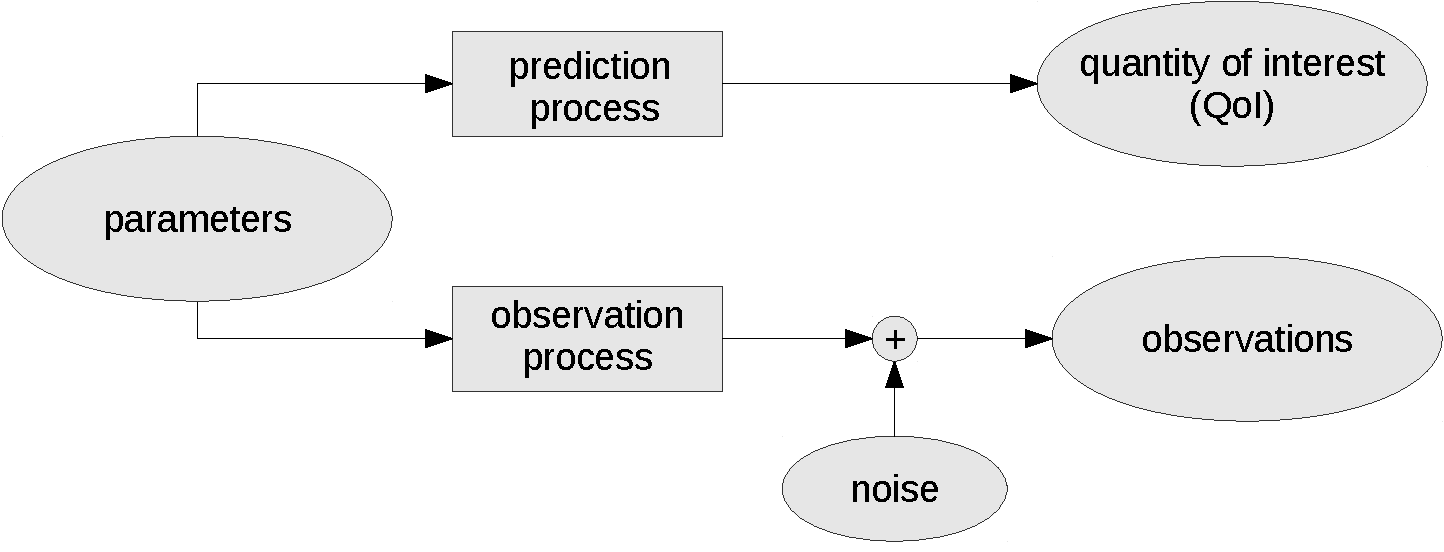
\includegraphics[width=0.8\textwidth]{intro/paramObsQoI.pdf}
\caption{The observation process, which often includes the forward model, relates the unknown parameters to the observations, which are also contaminated by noise. Once these parameters have been inferred from the observations, they are related to the QoI through the prediction process.}
\label{fig:qdI}
\end{figure}

In this spirit, one way to simplify the process of inferring the parameters is to represent the physical system to a coarser degree. A given physical system can be represented with varying degrees of fidelity by different models. A high-fidelity model may, for example, take into account more physical laws or be more finely discretized, and thus more accurately represent reality. However, a high-fidelity model is also usually more difficult to solve. Since solving the inverse problems generally requires many evaluations of the forward model, it may be cheaper to use a lower-fidelity model. In addition, the inverse problem is often ill-posed without regularization; it may be the case that even if one were to use the high-fidelity model, the additional resolution (in space-time and/or physical laws) of the high-fidelity model might not even be informed by the observations. Thus, it may not be necessary to infer the parameters using the expensive, high-fidelity model in order to accurately calculate the QoI. Just as we manage models to control the error in QoI predictions from solving the forward problem, for example through mesh adaptation, our research here aims to manage the fidelity of modeling choices in solving the inverse problem, so as to achieve a desired level of accuracy in the QoI prediction, without necessarily resolving the parameters accurately. We adaptively form a mixed-fidelity model with which we solve the inverse problem by using models of different levels of fidelity in different parts of the domain.

In the next section, we describe existing work on goal-oriented approaches and multifidelity modeling.

%------------------------------------------------------------------------------%
\section{Previous Work}  %\label{sec:xx}
%------------------------------------------------------------------------------%

In this section, we describe previous work, first on goal-oriented approaches and then on multifidelity modeling.

%------------------------------------------------------------%
\subsection{Goal-Oriented Approaches}
%------------------------------------------------------------%

Especially in engineering contexts, the ultimate goal of running a forward simulation or inferring parameters is to calculate some low-dimensional quantity of interest; the exact states or parameters may not otherwise be of interest. Goal-oriented approaches prioritize accuracy in the QoI over accuracy in the states and/or parameters. 

In the context of the forward problem, methods for goal-oriented mesh-refinement using adjoints are described in \cite{PrudOden99,VendDarm00,BecRann01}; an a posteriori error estimate in an output functional is derived, and this estimate is used to guide adaptive mesh-refinement. A framework for automated mesh-refinement to calculate a QoI to a prescribed accuracy is described in \cite{Yano12}. In \cite{OdenPrudetal06}, a method using adjoints for the goal-oriented forward problem is described; however, instead of targeting adaptive mesh refinement, the method adaptively divides the domain into subdomains where models describing different scales are applied. 
%read VendDarm00 for the lulz?

Work has also been done on goal-oriented methods for the inverse problem. Mesh-refinement in the goal-oriented inverse problem\footnote{What we refer to as the goal-oriented inverse problem is referred to as the problem of model calibration in \cite{BecVex05}.} is addressed in \cite{BecVex05}; in this work, Becker and Vexler derive an a posteriori estimate of the error in the QoI caused by discretizing the infinite dimensional inverse problem, and this error estimate is used to adaptively refine the mesh. In \cite{LiebWill13}, Lieberman and Willcox describe, for a discretized linear inverse problem, a low-dimensional subspace of the parameter space that is both informed by observations and informative to the QoI; this subspace is used to produce a low-dimensional map from the observations directly to the QoI, sacrificing accuracy in the inferred parameters for accuracy in the QoI that is computed from them.

%goal-oriented DoE from marzouk?
	%goal-oriented-ness seems to be not the focus of http://arxiv.org/pdf/1108.4146v3.pdf, but can be incorporated into utility function
%------------------------------------------------------------%
\subsection{Mixed-fidelity Models} \label{sec:multFid}
%------------------------------------------------------------%

A particular physical system can be represented with varying degrees of fidelity by different models. Often a lower-fidelity model will be cheaper to solve. However, it will also describe reality to a lesser degree of accuracy; it may include fewer physical laws (for example, the Euler equations ignore viscosity) or describe phenomena at a coarser scale (for example, a model of linear elasticity does not treat individual atoms). A mixed-fidelity model can combine higher- and lower-fidelity models in a way so as to be more tractable than the high-fidelity model, while maintaining accuracy.

Two main strategies exist for combining models: hierarchical and concurrent methods. Hierarchical methods (also known as information-passing or sequential methods) take the results of a simulation using the high-fidelity model and use them to inform a lower-fidelity model that is used globally (for example, modeling the molecular structure of a material to determine parameters for constitutive equations \cite{Haoetal03}). Concurrent methods simultaneously solve the high-fidelity model in some small portions of interest of the domain and the low-fidelity model in the remainder of the domain; for example, in \cite{Khareetal08} atomistic models capable of describing bond-breaking behaviors are applied to small clusters of atoms in regions relevant to the formation of fractures, while a continuum model is applied in the rest of the domain.

In our approach, we focus on concurrent methods of combining models. In general, the different models need not depict different scales. For example, in \cite{vanOpstaletal15} a mixed-fidelity model is formed by dividing the domain into subdomains where either the linear Stokes equation (low-fidelity) or the nonlinear Navier-Stokes equation (high-fidelity) is solved, based on an a posteriori estimate of the error in a QoI. The different models also need not represent different physical phenomena. For example, in \cite{LucKinBer02}, the domain is decomposed into regions with and without shocks, and a reduced-order model is developed for each region independently and later combined; in \cite{AntHein10}, balanced truncation model reduction is applied to the part of the domain outside of where the optimization variables are located in order to reduce the overall cost of a forward solve. The manner in which the different models are interfaced is problem-dependent; in \cite{Abra98, AlexGarTar02}, a ``handshake'' region is used to couple concurrent particle and continuum models, and in \cite{AlexGarTar02}, interface coupling models are introduced to reconcile uncertainties in the different models.

%hierarchical vs concurrent multi models- have lf-hf-mf cartoon here?
	%also apparently HF+LF models are combined by having the HF models generate numerical observations to use as training for reduced basis models

%idea of most-complex \neq best? occam's razor thing from all-hands...we may define HF as "best" for getting QoI, but it might not necessarily be the hardest to work with...

%------------------------------------------------------------------------------%
\section{Thesis Objectives}  %\label{sec:xx}
%------------------------------------------------------------------------------%

We aim to combine the ideas in goal-oriented methods for inverse problems, and goal-oriented model adaptivity approaches for forward modeling. The objective of this work is to formulate a method that allows one to systematically manage the use of multiple models in the context of the goal-oriented inverse problem, so as to minimize the error in a QoI prediction. To do this, we first assume that solving the inverse problem with the highest-fidelity model would result in the most accurate QoI, but that solving this inverse problem is prohibitively expensive. We derive an estimate for the error in the QoI from inferring the parameters using a lower-fidelity model. This estimate can be localized to individual elements, and the element-wise decomposition can then be used to guide the formation of mixed-fidelity models with which to solve the inverse problem, while minimizing the error in the QoI. This process is illustrated in Figure \ref{fig:lfhfmf}.

\begin{figure}[h]
\centering
\begin{subfigure}[b]{0.32\textwidth}
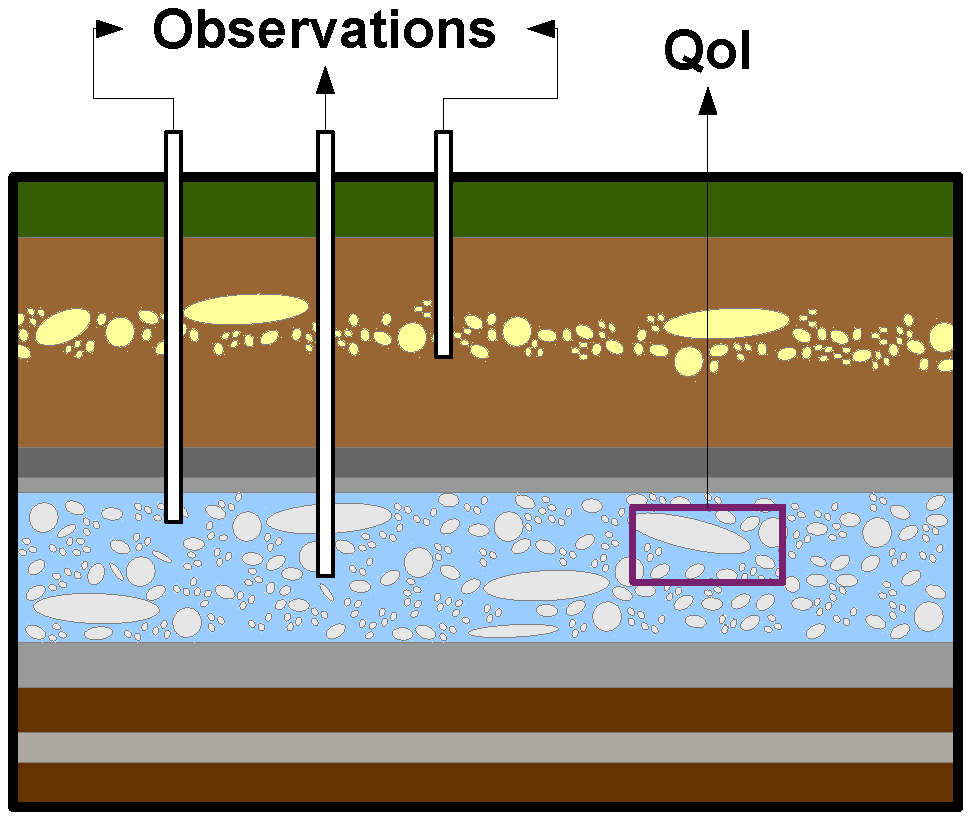
\includegraphics[width=\textwidth]{intro/hf.pdf}
\caption{High-fidelity}
\label{subfig:hf}
\end{subfigure}
\begin{subfigure}[b]{0.32\textwidth}
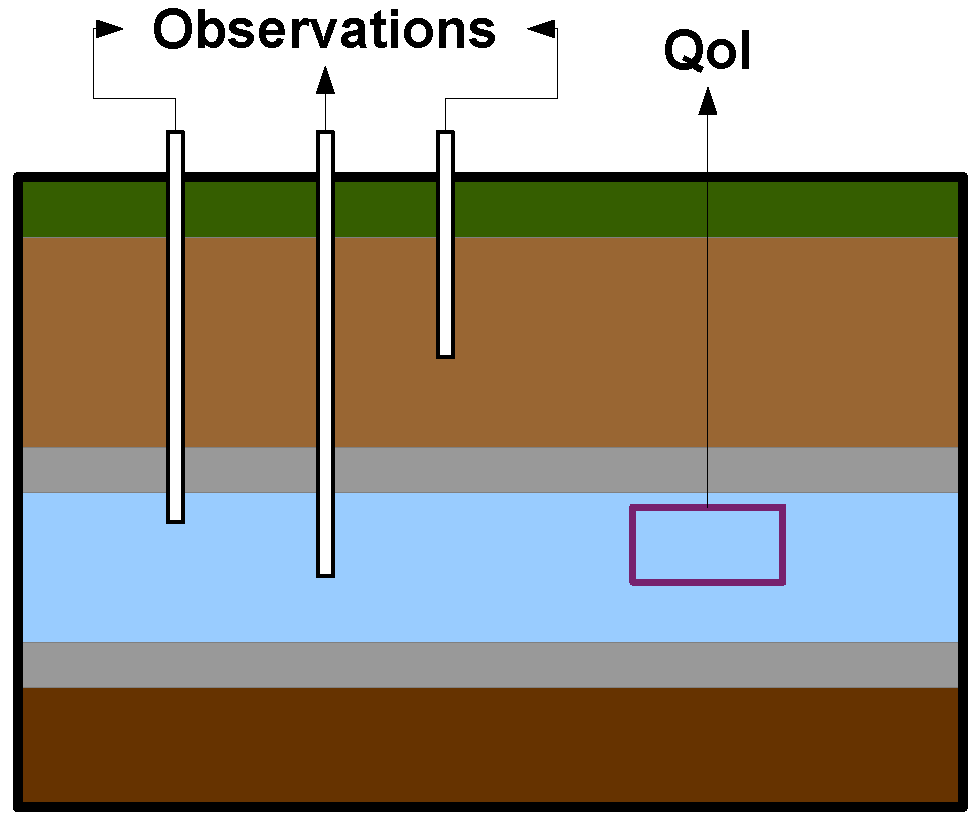
\includegraphics[width=\textwidth]{intro/lf.pdf}
\caption{Low-fidelity}
\label{subfig:lf}
\end{subfigure}
\begin{subfigure}[b]{0.32\textwidth}
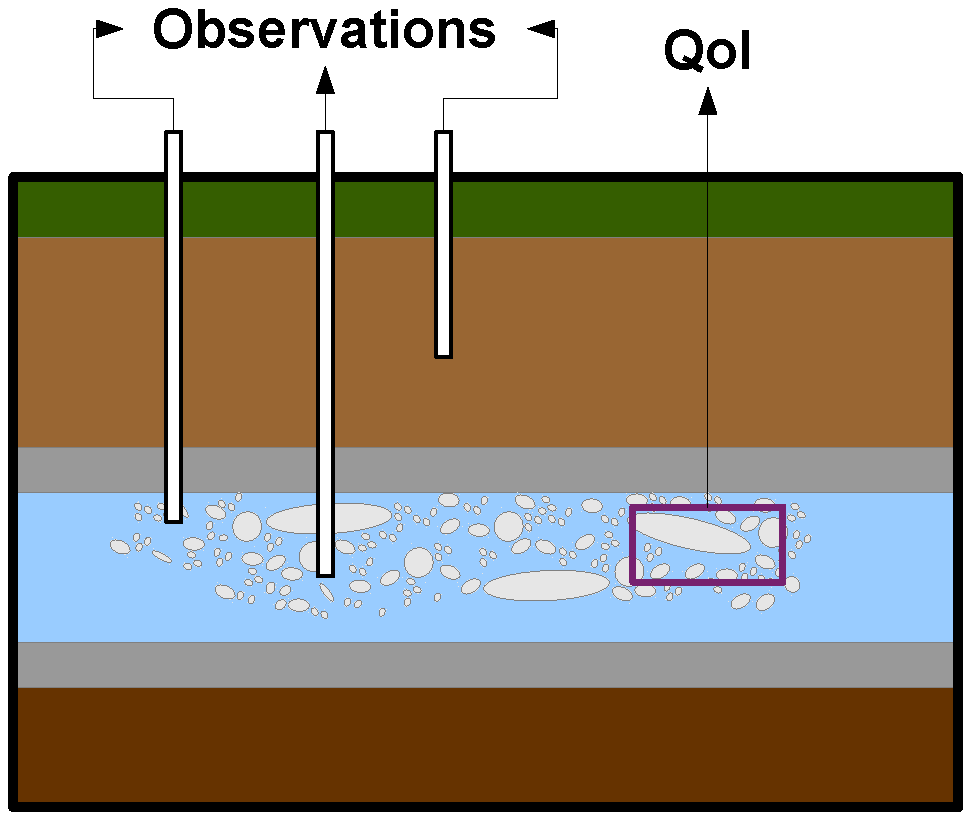
\includegraphics[width=\textwidth]{intro/mf.pdf}
\caption{Mixed-fidelity}
\label{subfig:mf}
\end{subfigure}
\caption{For a given QoI (e.g. average concentration in a region of an aquifer) and a set of observations (e.g. concentration measurements from wells), solving the inverse problem with a mixed-fidelity model (\subref{subfig:mf}), formed by using the high-fidelity (\subref{subfig:hf}) and low-fidelity (\subref{subfig:lf}) model in different parts of the domain, may give a QoI estimate with low error relative to that obtained from inferring the parameters with the high-fidelity model.}
\label{fig:lfhfmf}
\end{figure}

%------------------------------------------------------------------------------%
\section{Thesis Outline}  %\label{sec:xx}
%------------------------------------------------------------------------------%

In Chapter \ref{chap:form}, we define the goal-oriented inverse problem, derive an a posteriori error estimate for the QoI, and discuss its use for model adaptivity in the context of the goal-oriented inverse problem. In Chapter \ref{chap:results}, we apply the error estimate to adaptively form a mixed-fidelity model for two-dimensional convection-diffusion-reaction examples. In Chapter \ref{chap:conc}, we give a summary of the thesis, and suggest directions for future work.

